\section{System-level modeling}
\label{sec:esd-modeling}

% Context is a competitive environment, where any tool can make a difference
Electronic design world is highly competitive, especially automotive.
Vital to design products as fast as possible, with lowest possible costs, while guaranting quality.
On the other hand, electronics systems are complex to design and are almost never completely fullfill their specification at the first manufacturing round.
As design progresses and the project moves on in the design cycle, every redesign and modification becomes exponentially more costly.
For instance, modifying properties of a few transistors inside an integrated circuit during the early design phase comes almost for free.
A few minutes for a designer to make the changes.
However, if this change must be done after a first tapeout, then it costs a few minutes to a designer to make the changes, plus modifications of the layout of the product, setup of a new tapeout, tapeout manufacturing cost, a few months of manufacturing time, testing time for the new part.
To remain competitive, the amount of design-manufacturing phases must be kept to a bare minimum, ideally to a single pass.
In this context, any tool capable of detecting early issues, enabling to prevent them before manufacturing, is highly valuable.

%TODO: Schema with design cycle + cost increase at each step

% Simulations are vital
Electrical simulations are the corner-stone of modern, computer-aided electronic design.
They constitute a fundamental tool used massively in integrated circuits and systems development.
Silicon-manufacturing companies put a lot of effort to develop highly accurate models of their integrated technologies.
In those environments, accuracy of standard analog simulations is rightfully taken for granted.
For electrostatic and electromagnetic simulations though, the situation is different.
By nature, electrostatic discharge are very fast and highly non-linear signals.
Those events occupy a much larger frequency spectrum than waveforms usally met in standard analog simulations.
It is essential to verify the accuracy of models and simulations.
Models must be validated against actual measurement data, and in many different test conditions, including powered and unpowered conditions.

% Need to simulate from source to input for soft-failure analysis
In this chapter, a methodology for building electrical ESD models is proposed, in order to simulate waveforms from the ESD source to an integrated circuit pin.
This is a preliminary step for enabling simulation of soft-failures inside the chip.
The proposed methodology is modular and offers to reuse models between common devices found in ESD laboratories.
A typical ESD test setup comprises equipments such as DC sources, oscilloscopes, and stress generators.
Equipments are connected together with wires, coaxial cables, twisted wire pairs, etc.
The integrated circuit under test is often soldered onto a printed circuit board.
\gls{PCB}s usually host multiple kind of discrete devices, such as passive devices, ESD protections, common-mode chokes, relays, etc.
Components are connected together by metal tracks.
The goal of the proposed methodology is to build a library of all those elements, from lab equipments down to tiny discrete components.
Each model of the library will be qualified independently with individual characterization and comparison with its model.

% Assemble models together to build the complete thing
%TODO: Etoffer
After the library is constructed, models can be connected together to simulate the entire system.
The topology of the system serves as a blueprint for connecting models.

\subsection{Transmission line}

% Cables and delays identified as important for esd sims - because of similar order of magnitude
Cables are critial elements in any \gls{esd} test setup.
They introduce significant propagation delays in regard of the duration of an electrostatic discharge.
A 50\textOmega{} coaxial cable has a propagation ratio of approximately 5 ns/m.
In a laboratory, it is common to find cables of tens of centimers to a couple of meters long, resulting in delays between 1 ns and 10 ns.
As a comparison, the scale of an electrostatic discharge is a few hundred nanoseconds.
Both values are near the same order of magnitude and a large impact from cables on the simulation can logically be expected.
Cables, microstrip lines, wires and electrical propagation media behave as transmission lines.
Transmission lines were originally analysed by J. Maxwell, L. Kelvin and O. Heavyside and a huge amount of studies on the topic are available in the litterature \cite{branin-tl-ref, hf-coax,lossy-tl,emc-analysis-tl}.

% Cables can be a source of oscillations
Cables can also be a source of ringing oscillations if the circuit contains impedance mismatches, which is often the case.
Oscillation period is directly related to the cable length.
In this situation, a delay even less than 1 ns can have a strong impact on waveforms.
Therefore, coaxial cables, long \gls{pcb} traces and any element that generates a significant delay superior to the nanosecond should be modelled.

% Emphasize that a good line model is essential given how often the TLP is used for analysis in the ESD field
Transmission line pulsing was used extensively during this study.
As a remainder, it consists primarily in the discharge of a coaxial cable.
Thus, proper modelling of coaxial cables is useful in that regard as well.

% model delays with lossless TL
Transmission lines are characterized by their characteristic impedance, supposedly constant on the entire line.
It is determined by its cross-sectional dimensions and constituting materials.
For coaxial cables, common characteristic impedances are 50\textOmega{} or 75\textOmega{}.
This value is equivalent to the resistance that could be measured statically between outer and inner conductors for an \textbf{infinitely long} transmission line.
All transmission lines are lossy, meaning that some a part of the incoming power traversing it is dissipated.
In most cases though, losses are very small and negligible, and the line is considered lossless.
The behavior of the line is also frequency-dependant.
Losses, characteristic impedance and other properties can change above certain frequencies.
For frequencies below a GHz, most cables and metal strips can be correctly approximated by a lossless and non frequency-dependant line.

% How is a transmission line mathematically modelled
Physically, a transmission line can be seens as a succession of infinitely small unit elements.
Each element is modeled by an inductance \textdelta{}L, a capacitance \textdelta{}C and sometimes a leakage resistance or conductance.
Those unit values are directly related to the characteristic impedance Z\textsubscript{c} as described in Eq. \ref{eq:characteristic-impedance}.
\gls{Zc} is the also expressed as the ratio of voltage and current of a single wave propagating along the line.

\begin{equation}
Z_{c} = \sqrt{\frac{\delta L}{\delta C}}
\label{eq:characteristic-impedance}
\end{equation}

\subsubsection{Distributed model}

% Distributed model
The most popular line model in the ESD field is based on lumped capacitance and inductance.
The model is a series of lumped L-C networks as illustrated in Fig. \ref{fig:dis-line-model}.
Values for the element can be computed from the characteristic impedance \gls{Zc} with Eq. \ref{eq:characteristic-impedance}.

\begin{figure}[!h]
  \centering
  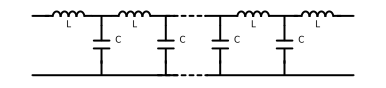
\includegraphics[width=0.7\textwidth]{src/2/figures/lc_ladder.pdf}
  \caption{Electrical distributed LC ladder model of a lossless transmission line}
  \label{fig:dis-line-model}
\end{figure}

\begin{equation}
\delta t = \sqrt{\delta L.\delta C}
\label{eq:unit-delay}
\end{equation}

% A string of unit elements form the total model
Each element induces a propagation delay \textdelta{}t, whose values can be computed from the unit inductance and capacitance with Eq. \ref{eq:unit-delay}.
In a string of connected unit elements, the individual delays add up.
With enough elements, the delay and behavior of the complete cable is reproduced.

% Tradeoff between amount of elements and
During modelling, it is tempting to take large values for \textdelta{}L and \textdelta{}C, to get a large unit delay.
Doing so reduces the amount of unit elements, and speeds up the simulation.
However, there is a tradoff between the delay of the unit element and the accuracy of the simulation.
A smaller unit delay increases accuracy of the model at large frequencies, but more elements are required for the total cable, resulting in longer simulation times.
On the other hand, a larger unit delay reduces the bandwidth of the model, which may be unsuitable for accuracy, even if simulation times are improved.

% How to calculate the unit values ?
By resolving the equation system constituted \ref{eq:characteristic-impedance} and \ref{eq:unit-delay}, it is possible to extract formula for L (Eq. \ref{eq:unit-inductance}) and C (Eq. \ref{eq:unit-capacitance}).
Values depend on the characteristic impedance Z\textsubscript{C}, the total cable delay \textDelta{}t and the amount N of lumped elements in the model.

\begin{equation}
L = \frac{Z_{C}.\delta t }{N}}
\label{eq:unit-inductance}
\end{equation}

\begin{equation}
C = \frac{\delta t}{N.Z_{C}}}
\label{eq:unit-capacitance}
\end{equation}

% Perks and disavantages
The distributed model supports easily lossy transmission lines by adding a unit resistance or conductance between signal and ground, or in series with the signal.
On the other hand, this model does not scale well as cables get longer.
To keep the same bandwidth with a longer cable, the only solution is to increase the element count, resulting in longer simulation time.
Also, this model will always be bandwidth limited, otherwise it would require an infinite amount of infinitely small elements.

\subsubsection{Two-port network model}

% Behavioral model
The two-port network model described by H. Branin \cite{branin-tl-ref} is a much better alternative to the distributed model.
It can describe efficiently and with great accuracy the behavior of uniform lossless transmission lines.
The model is constituted of two voltage-controlled voltage sources and two resistors (Fig. \ref{fig:beh-line-model}).
Compared to the distributed model, the behavioral model has by design an infinite bandwith, and is extremely fast to simulate.
It also is constant in complexity, because the simulation time is independant of the cable's delay or required bandwidth

\begin{figure}[!h]
  \centering
  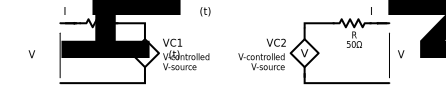
\includegraphics[width=\textwidth]{src/2/figures/behavioral_line_model.pdf}
  \caption{Electrical behavioral model of a lossless transmission line}
  \label{fig:beh-line-model}
\end{figure}

Equations \ref{eq:beh-line-1} and \ref{eq:beh-line-2} describe the behavior of the voltage-controlled voltage sources.

\begin{equation}
V_{C1}(t) = V_{2}(t - \Delta t) + Z_{C}.I_{2}(t - \Delta t)
\label{eq:beh-line-1}
\end{equation}

\begin{equation}
V_{C2}(t) = V_{1}(t - \Delta t) + Z_{C}.I_{1}(t - \Delta t)
\label{eq:beh-line-2}
\end{equation}

% Explain the equations
Z\textsubscript{C} is the characteristic impedance of the line and \textDelta{}t the propagation delay between both ports.
Overall, the equations describes a system where voltage and current at both ports are defined by the combination of a forward travelling wave and a backward travelling wave.
An example implementation in VHDL-AMS is provided in Listing \ref{lst:tline}.

\begin{code}
\inputminted[frame=single]{VHDL}{src/2/snippets/tline.vhdl}
\caption{Transmission line behavioral VHDL-AMS model}
\label{lst:tline}
\end{code}

\subsubsection{Comparison}

% Compare both models to know which one is preferrable
Simulations are ran to compare both models.
The setup is given in Fig. \ref{fig:lines-testbench} and consists in injecting a rectangular pulse with a risetime of 1 ps into a load through the modelled transmission line.
Different load values are employed to observe the performance and accuracy of each model.
The transmission line to model has been chosen to a delay of 100ns and a characteristic impedance of 50 \textOmega.
Both values correspond to the cable usually employed in a transmission line pulsing generator and are thus very realistic.

%TODO: Simulation with 10

\begin{figure}[!h]
  \centering
  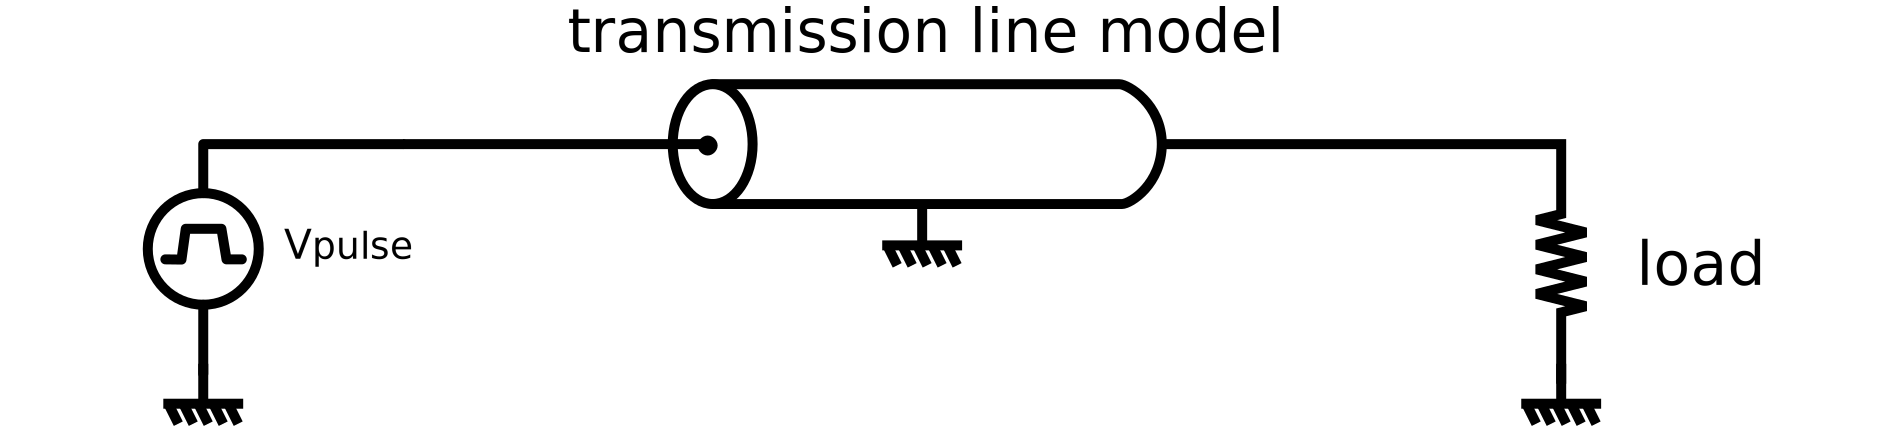
\includegraphics[width=0.8\textwidth]{src/2/figures/tline_validation_setup.pdf}
  \caption{Line model validation testbench}
  \label{fig:lines-testbench}
\end{figure}

Overall, the behavioral model outperforms the distributed model for representing a perfect transmission line.
It reproduces exactly the 1ps risetime on the load in all configurations (Fig. \ref{fig:lines-simulations}).
The distributed model is either not as accurate or much slower to simulate.

\begin{table}[!h]
\centering
\begin{tabular}{@{}lllll@{}}
\toprule
amount N         &  10           & 100        &  1000      &   10000    \\ \midrule
simulation time  &  15 ms        & 170 ms     &  7.5 s     &   135 s    \\
increase ratio   &  -            & x10        &  x44       &   x18      \\
\bottomrule
\end{tabular}
\caption{Impact of the amount of unit elements on the simulation times}
\label{tab:tline-impact-simulation-time}
\end{table}

For good accuracy, individual delay must be 2 or 10 times smaller than the shortest rise time.
Also, simulators with variable timestep have trouble reproducing appropriately oscillating events.
Simulated period is often wrong compared to what is mathematically expected.
Oscillations also force the simulators to fall back to the smallest timestep, considerably increasing simulation times.
To simulate a 100 ns TLP with a 100 ps risetime using the distributed model, it would require unit elements with a of 10ps.
10000 elements would be required to model the line, which is rather important and increases simulation time.
And even with 10000 elements, resolution is still to larg to obtain a clean risetime \ref{fig:lines-simulations}.

\begin{figure}[!h]
  \centering
  \includegraphics[width=0.3\textwidth]{src/2/figures/tline_models_comparison.pdf}
  \caption{Lumped versus two-port models comparison in simulation}
  \label{fig:lines-simulations}
\end{figure}

In conclusion, the two-port model should always be preferred over the lumped model.
This is obviously the approach used for all transmission line modelling presented in this document.

\subsection{Passive devices}

% Passive devices are everywhere
Discrete passive devices are highly widespread at board level.
Not a single PCB without discrete on it.
Not integrated on silicon because most of the time it is cheaper to use external devices instead of consuming large silicon areas to integrate them.

% Limitations of passive devices
Properties of passive devices such as capacitors, resistors and inductors change in \gls{esd} conditions \cite{capa-esd-cz}.
For large transient amplitudes above nominal range and high-frequencies, their nominal values easily vary by an order of magnitude.
At frequencies above a few MHz, the parasitic devices play an important role and make the device ineffective at some point.
For instance, capacitors exhibit an inductive behavior for sufficiently large frequencies.

% In what frequency range are ESD active, and are those limitations in effect
Electrostatic discharges have been characterized in the frequency domain in \cite{fft-esd}.
It concerns air discharges and non-shielded discharges that radiate heavily.
The spectrum of the IEC 61000-4-2 standard \cite{iec61000-4-2} was recorded.
It is shown that the majority of the frequency content is below 1GHz, with important magnitudes until tens of MHz.
Like indicated previously, this is the frequency range where parasitic behavior is important.
Therefore for \gls{esd} simulations, passive devices require models that take those parasitic devices into account.

% Not all device need parasitic device modelling
In practice, it was found that only some passive devices in a system have a notable impact on the waveform at high-frequencies.
For others, using a regular electrical model is sufficient.
Decoupling capacitors were noticed to require parasitic device modelling.
Since they are connected between a voltage reference (supply voltage) and a reference (ground), they have a strong impact on the disturbance waveforms that an \gls{ic} pin is exposed to.
Passive device models working at frequencies below 1GHz are given in Fig. \ref{fig:rlc-esd-models} for inductors, resistors and capacitors.

\begin{figure}[!h]
  \centering
  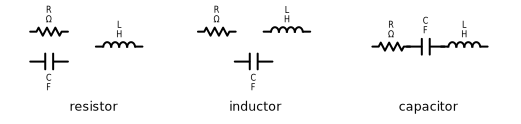
\includegraphics[width=\textwidth]{src/1/figures/rlc_models.pdf}
  \caption{High-frequency (< 1GHz) models for resistor, capacitor and inductor}
  \label{fig:rlc-esd-models}
\end{figure}

% How to tune those models
Those models are easily parameterized.
Values can be extracted with an impedance meter capable of measuring impedances to at least 100 MHz.
Fig. \ref{fig:frequency-response-capa} displays the magnitude and phase versus frequency of a 6.8 nF \gls{smd} capacitor.
The capacitor exhibits a perfect behavior up to 45MHz.
The slope of the curve below 45 MHz is directly related to the capacitor value (see Equation \ref{eq:capacitor-impedance}).
Below 45 MHz, the phase has a value of $-90$ degrees, corresponding to the theory.

%TODO: Check this equation
\begin{equation}
\delta M/ \delta f = C. \omega = 2.\omega .C.f
\label{eq:capacitor-impedance}
\end{equation}

% What are the parasitic devices in this curve
At the resonant frequency, the capacitor is equivalent to a non-ideal short-circuit, basically a low-value resistor.
This resistor, also called \gls{esr}, is both a parasitic device and the series resistance in the high-frequency model presented earlier.
Beyond 45 MHz, the capacitor behaves as an inductor.
The phase shift is the one of an inductor at $+90$ degrees.
This second slope is determined by the parasitic inductor value (see equation \ref{eq:inductor-impedance}).
In conclusion, the values for parasitic inductor and resistor can be computed very easily from a measurement.

\begin{equation}
\delta M/ \delta f =  -L.\omega = -2.\omega .L.f
\label{eq:inductor-impedance}
\end{equation}

\begin{figure}[!h]
  \centering
  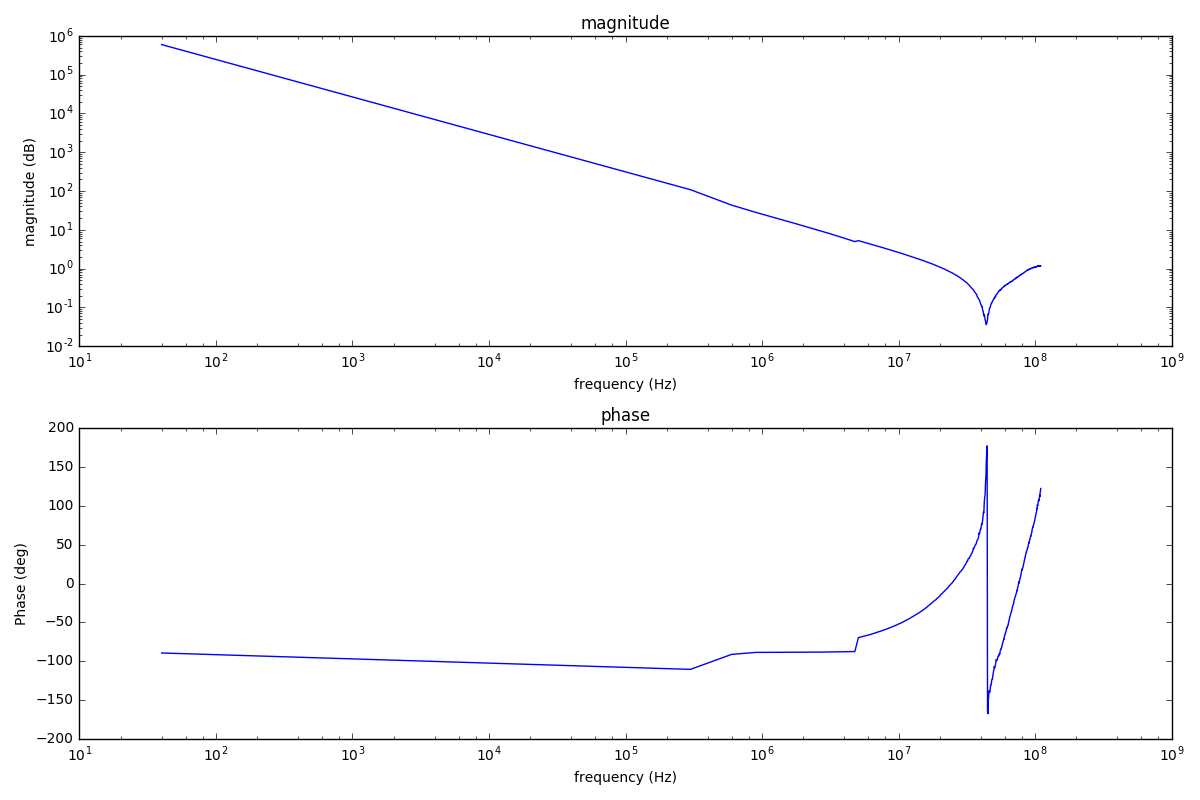
\includegraphics[width=0.3\textwidth]{src/1/figures/capa_hf_response.png}
  \caption{Frequency response of a 6.8nF capacitor}
  \label{fig:frequency-response-capa}
\end{figure}

% Impact of dimensions on parasitic values
%TODO: Quote fabien ? Or find reference
In the case of capacitors, for a given package, first observations tend to show few variations for the parasitic inductance, even with capacitors of different values and sizes.
The parasitic inductance seems mostly related to the kind of package, and measured values are between 1nH and 5nH.
This observation tends to indicate that there is no need to characterize every single passive device.
Instead, a global parasitic model per package should suffice.

% Non-linear high power behavior
%TODO: Quote fabien
%TODO: Find articles that show non-linear behavior
So far, only the frequency-related behavior was detailed.
For high power and amplitudes, most passive devices also suffer of nominal ratings variations.
\gls{mlcc} are concerned about this phenomenon \cite{capa-esd-cz}, where the capacitance decreases at high voltages.
On the contrary, capacitors built with the X7R technology are much most resilient in high regime conditions and exhibit little variations.

% Conclusion
%TODO

\subsection{ESD protections}
\label{esd-protection-modelling}

%TODO: A etoffer

% Diodes
Diodes and \gls{tvs} are frequently studied devices in the \gls{esd} field \cite{modelling-diode-esd, esd-diode-compact-model, tvs-modeling}.
Multiple modelling methods exist, such as behavioral and compact models.
Most studies target silicon-level devices, but a few also interested in board-level active device modelling.

Behavioral model from laas
State machine
convergence issues
triggering delay not taken into account (reference Fabien's work) ?



\subsection{Common mode filter}

% Common mode choke
Common mode choke are frequently encountered in electronic systems to protect inputs and supplies in particular \cite{cmc-for-emc-protection, cmc-esd, alternative-cmc-emi-noise}.
Unlike regular RC-network filtering, chokes isolate from common mode disturbances where both signal and ground reference voltages shift.
Chokes are frequently used for reducing emmission in \gls{emc} tests, and increasing immunity of a system to conducted disturbances.
CMF are modeled for ESD in \cite{usb2ESDProtection}

%TODO: Give electrical model

quote:
Common mode filters have the particularity to exhibit
different insertion impedance according to the
excitation modes (Fig. 10). For differential signals,
CMF will present a small impedance while a large
impedance will be presented for common mode
signals, overall making them effective in a
differential interface to filter out common noise while
preserving integrity of the differential signal
(DP,DM).

linear vs non-linear model

\subsection{Ferrite beads}

%TODO: Similar to CMF ?
%TODO: description and function

Ferrite beads are modeled for ESD in  \cite{mixedModeESDSims}

%TODO: Give electrical model and picture

\subsection{Modeling techniques}

% Assembling models is one step, but need to be cautious on the results
The modeling method consists in connecting together models of devices that physically exist.
To reach good agreement between simulation and measurement, some phenomena must also be taken into account.
They can strongly impact waveforms.
In particular, propagation and reflection phenomena play a key role at the nanosecond timescale with macro-scale systems.
They are completely ignored in standard time-domain electrical simulations and analysis, because the time constants involved are much shorter than the typical timescale.
For instance, a combination of a propagation delay with reflected wave sometimes leads to dampened oscillations with a period in the range of a few nanoseconds that last for tens of nanoseconds.
In comparison, most analog functions in the automotive field have time constants above tens of microseconds, that is to say 5 orders of magnitude longer.
In those simulations, nanosecond scale event can be purely and simply ignored.
However, in \gls{esd} simulations, nanosecond scale event are important because the waveforms last for the same order of magnitude.
%TODO : Speak about the relation between the propagation delay time constants involved in regard of the dimensions of the system

% Propagation phemenon
%TODO
Propagation is a phenomenon that always occurs but is negligible over a few tens microseconds.
Below that timescale it must be taken into account because it has a major impact on the waveforms.
This is due to the fact that observation times are in the same range than electrical wave propagation times.

% Reflection phenomenon
%TODO
Reflection happens when an electrical wave propagates and reaches a point where two propagation media are mismatched (two coaxial cables of different characteristic impedance for example).

% Combined impact
%TODO
These two effects and in combination can impact waveform in some specific scenario

% Measurement artifact
Spike visible on measurements but is just an artifact
Caused by a delay between an intended measurement point and where the measurement is actually performed
Delay because of a cable for instance
Setup given in Fig \ref{fig:setup-measurement-spike}

\begin{figure}[!h]
  \centering
  \includegraphics[width=0.3\textwidth]{src/1/figures/setup_measurement_spike.pdf}
  \caption{Typical setup causing a measurement artifact}
  \label{fig:setup-measurement-spike}
\end{figure}

The process that generates this measurement glitch starts with the injection of a fast rectangular pulse.
The pulse propagates towards point A (step 1).

\begin{figure}[!h]
  \centering
  \includegraphics[width=0.3\textwidth]{src/1/figures/spike_generation_1.pdf}
  \caption{Spike generation - step 1}
  \label{fig:spike-step-1}
\end{figure}

At the moment it reaches A, the capacitor load is not immediately visible.
It is “hidden” from point A by the short delay.
Thus, the voltage rises, depending at this point only on the characteristic impedances of the cables.
A part of the pulse propagates towards the load and a part toward Vout (depending on the impedance ratio) (step 2).

\begin{figure}[!h]
  \centering
  \includegraphics[width=0.3\textwidth]{src/1/figures/spike_generation_2.pdf}
  \caption{Spike generation - step 2}
  \label{fig:spike-step-2}
\end{figure}

The impulse reaches then the load (step 3), and propagates back toward A, settling the voltage at A to
V – (V – Vload) = Vload (forward travelling wave minus reflected wave from load) (step 3).
The capacitor is supposed to be charging at constant current, voltage rises following a linear curve.

\begin{figure}[!h]
  \centering
  \includegraphics[width=0.3\textwidth]{src/1/figures/spike_generation_3.pdf}
  \caption{Spike generation - step 3}
  \label{fig:spike-step-3}
\end{figure}

Now the voltage at point A is defined by the load.
However before that, the voltage rose and generated a peak that will hit Vout after a delay.
This peak preceding the capacitor charge is detailed on figure \ref{fig:spike-step-4}.
The amplitude is exaggerated for illustration purposes

\begin{figure}[!h]
  \centering
  \includegraphics[width=0.3\textwidth]{src/1/figures/spike_generation_4.pdf}
  \caption{Spike generation - step 4}
  \label{fig:spike-step-4}
\end{figure}

In a more realistic situation, if the short delay is of the same order of magnitude than the pulse risetime, the generated peak will be a non-negligible fraction of the initial pulse amplitude.

\begin{figure}[!h]
  \centering
  \includegraphics[width=0.3\textwidth]{src/1/figures/spike_generation_5.pdf}
  \caption{Measured waveform}
  \label{fig:spike-step-4}
\end{figure}

% Unterminated cables
Because of propagation and reflection phenomena, elements that are normally ignored in standard simulations can no longer be neglected.
A perfect illustration of this point are cables connected to the circuit on one end, and left floating on the other end (or in high impedance)
In regular simulations, they can removed entirely.
With ESD simulations, they will induce oscillations and amplitude changes

\begin{figure}[!h]
  \centering
  \includegraphics[width=0.3\textwidth]{src/1/figures/setup_unconnected_cable.pdf}
  \caption{Typical setup causing oscillations}
  \label{fig:setup-unconnected-cable}
\end{figure}

%TODO: Rewrite completely
Transient current propagates toward the unconnected end
Reflects entirely at the high impedance termination
Comes back inside the circuit, absorbing a part of the initial current and supplying it later on.
The consequence is an undershoot followed by a delayed overshoot (fig. 15).
%TODO: Put a waveform ?

\gls{tlp} is a perfect example of an application exploiting an unterminated cable

% Feeding cables
%TODO: Talk about location of measurement point
Similarly, all cables on the propagation path (Fig. \ref{fig:setup-feeding-cable}) must not be neglected just because they are matched with the circuit.
The delay they introduce impacts greatly the waveforms.
TLP generators always require a cable to connect the load under test to the generator.
This connection cable plays a role in the final waveform.
In simulation, if omitted, the waveform is very rectangular and clean (Fig. \ref{fig:comparison-feeding-cable}).
When the cable is added, the presence of reflections with this delay changes quite a lot the waveform that now has an initial step between 00 and XX ns, with an amplitude corresponding to the TLP charging voltage and not the circuit operating point
XX ns corresponds exactly to (twice ?) the delay of the feeding coaxial cable.

\begin{figure}[!h]
  \centering
  \includegraphics[width=0.3\textwidth]{src/1/figures/setup_feeding_cable.pdf}
  \caption{Minimal TLP generator with feeding cable and a mismatched load}
  \label{fig:setup-feeding-cable}
\end{figure}

\begin{figure}[!h]
  \centering
  \includegraphics[width=0.3\textwidth]{src/1/figures/comparison_feeding_cable.png}
  \caption{Simulated waveform with and without feeding cable}
  \label{fig:comparison-feeding-cable}
\end{figure}

% Conclusion
%TODO: Detail
Beyond these particular examples, the idea is to be cautious about even short delays when assembling models from the library.
